\documentclass[tikz,convert={density=150,size=600,outext=.pdf},dvipsnames]{standalone}
\usetikzlibrary{shapes, calc, arrows, fit, positioning, decorations, patterns,
                decorations.pathreplacing, chains}
\usepackage{fontspec}
\setmainfont{CMU Serif}

\begin{document}
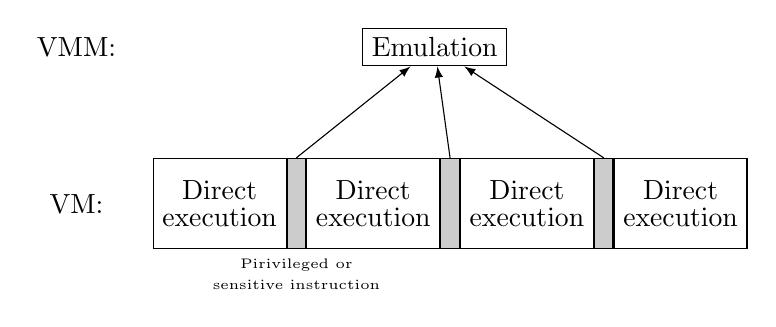
\begin{tikzpicture}[>=latex]
\node[] (VMM) {VMM:};
\node[draw, rectangle, right=3cm of VMM] (interpreter) {Emulation};

\node[below=1.5cm of VMM] (code) {VM:};
\node[draw, rectangle, right=0.5cm of code, minimum height=1.15cm] (de0) {\shortstack{Direct\\execution}};
\node[draw, fill=black!20, rectangle, right=0cm of de0, minimum height=1.15cm] (trap0) {};
\node[below=0cm of trap0] {\shortstack{\tiny{Pirivileged or}\\\tiny{sensitive instruction}}};
\node[draw, rectangle, right=0cm of trap0, minimum height=1.15cm] (de1) {\shortstack{Direct\\execution}};
\node[draw, fill=black!20, rectangle, right=0cm of de1, minimum height=1.15cm] (trap1) {};
\node[draw, rectangle, right=0cm of trap1, minimum height=1.15cm] (de2) {\shortstack{Direct\\execution}};
\node[draw, fill=black!20, rectangle, right=0cm of de2, minimum height=1.15cm] (trap2) {};
\node[draw, rectangle, right=0cm of trap2, minimum height=1.15cm] {\shortstack{Direct\\execution}};

\draw[->] (trap0.north) -- (interpreter);
\draw[->] (trap1.north) -- (interpreter);
\draw[->] (trap2.north) -- (interpreter);
\end{tikzpicture}
\end{document}
